% XCircuit output "outamp.tex" for LaTeX input from outamp.eps
\def\putbox#1#2#3#4{\makebox[0in][l]{\makebox[#1][l]{}\raisebox{\baselineskip}[0in][0in]{\raisebox{#2}[0in][0in]{\scalebox{#3}{#4}}}}}
\def\rightbox#1{\makebox[0in][r]{#1}}
\def\centbox#1{\makebox[0in]{#1}}
\def\topbox#1{\raisebox{-0.60\baselineskip}[0in][0in]{#1}}
\def\midbox#1{\raisebox{-0.20\baselineskip}[0in][0in]{#1}}
   \scalebox{0.7}{
   \normalsize
   \parbox{3.97396in}{
   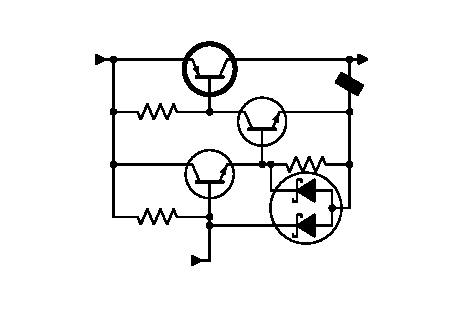
\includegraphics[scale=1.42857]{outamp}\\
   % translate x=708 y=296 scale 0.26
   \putbox{0.67in}{2.36in}{1.20}{\rightbox{\midbox{Power}}}%
   \putbox{0.67in}{2.19in}{1.20}{\rightbox{\midbox{Input}}}%
   \putbox{3.42in}{2.36in}{1.20}{\midbox{Power}}%
   \putbox{3.42in}{2.19in}{1.20}{\midbox{Output}}%
   \putbox{1.59in}{0.36in}{1.20}{\rightbox{\midbox{Control}}}%
   \putbox{1.59in}{0.53in}{1.20}{\rightbox{\midbox{From}}}%
   \putbox{1.59in}{0.19in}{1.20}{\rightbox{\midbox{Amplifier}}}%
   } % close 'parbox'
   } % close 'scalebox'
   \vspace{-\baselineskip} % this is not necessary, but looks better
